	LA GDT (\textit{Global Descriptor Table})  es una estructura de datos
que la arquitectura intel x86 utiliza para almacenar distintos descriptores
de sistema. En este trabajo sólo utilizamos 3 tipos de descriptores: El
primero y mas trivial es un descriptor nulo. El procesador produce
una excepción automáticamente cunado se intenta acceder a la posición cero
de la GDT. De esta manera el primer espacio de la tabla se rellena con
un descriptor nulo para evitar confusiones. Es decir que este descriptor
en realidad cumple una función accesoria, no modifica en nada el funcionamiento
del sistema. Sin embargo es muy cómodo que este ahí. El segundo tipo
de descriptor le corresponde a los descriptores de segmento. Los mismos
delimentan el tamaño y la ubicación de los segmentos, así como sus propiedades
(quién los puede acceder, que clase código hay adentro, etc, etc. Por último
se utilizaron descriptores de TSS para realizar el salto automático de tareas
(sobre esto vamos a hablar mas adelante con mayor profundidad, ahora sólo
se explicará la parte que concierne específicamente a la GDT).


\subsection{Segmentación flat}

	Como indica el enunciado todo el trabajo funciona con segmentación flat.
Esto significa dejar de lado la protección por segmentación armando 4 segmentos
que ocupen toda la memoria superpuestos entre si. Estos 4 segmentos son 2
con nivel de privilegio cero (máximo nivel de provilegios) y 2 con nivel de privilegio
3 (mínimo nivel de privilegios), y para cada nivel un segmento de código y uno
de datos.

	Por supuesto que esta práctica acarrea problemas, algunos de ellos graves
como por ejemplo que se pierde toda la protección por hardware brindada
por la segmentación. La contracara de esto es que se obtiene un entorno
mucho mas amistoso para programar, y la mayoría de la seguridad que se pierde
por la segmentación se puede recuperar utilizando de manera adecuado la paginación.

\subsection{Descriptores de segmento}

	Los descriptores de segmento se hardcodean en tiempo de compilación. Es decir
que en el mismo código la GDT ya contiene sus descriptores de segmento con
los parámetros adecuados. Es importante que esto se puede realizar exclusivamente
porque todos lo necesario para completar esos descriptores se conoce de antemano.
Esto en parte es una consecuencia de la segmentación flat.

	Una vez que el programa empieza a correr estos descriptores de segmento
no se vuelven a modificar. Se trabaja siempre los segmentos flat, por lo que no
hace falta modificar ni agregar nada. Quedan estáticos para siempre.

	Además de los segmentos flat se crea un segmento que contiene la memoria de video.
Este segmento se utilizó con fines didácticos en un principio, pero luego
todas las funciones de video que se utilizan a lo largo del trabajo acceden
a la memoria de video por medio del segmento flat de datos de nivel 0.

\subsubsection{Atributos descriptores de segmento}


\begin{figure}[h]
\begin{center}
  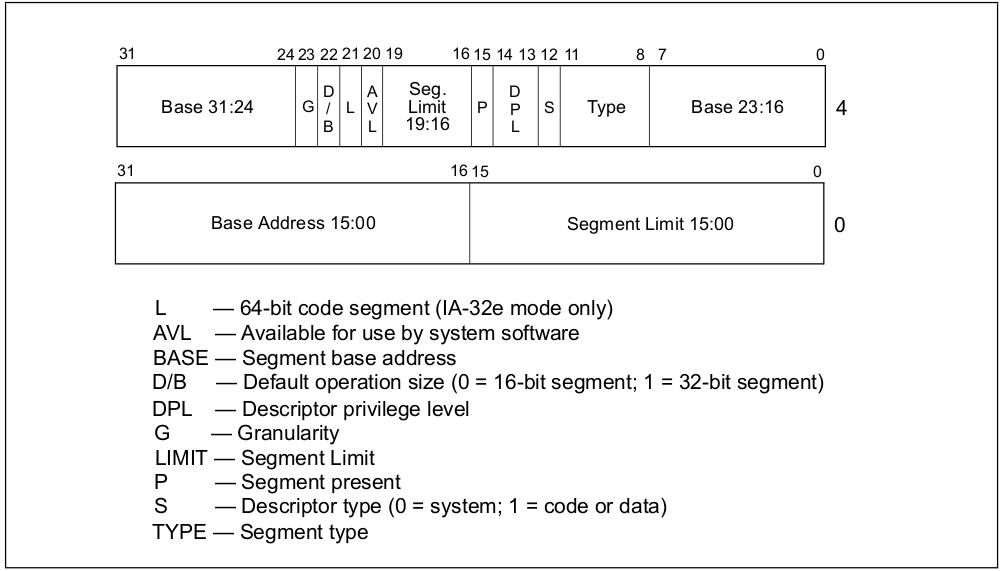
\includegraphics[scale=0.3]{secciones/dibujitos/descriptorDeSegmento.png}
\end{center}
\caption{Descriptor de segmento}
\label{fig:descriptorDeSegmento}
\end{figure}


	

\subsection{Descriptores de TSS}

	Para los descriptores de TSS se eligió otra dinámica. Las TSS se encuentran
ubicadas en un arreglo de TSS que se crea dinámicamente en tiempo de ejecución, por lo
que en el momento de la compilación no se sabe el lugar donde va a estar y por lo tanto
no se puede hardcodear esa dirección.

	Lo que se hizo, entonces, fue agregar los descriptores de TSSde manera dinámica en tiempo
de ejecución. Para esto se crearon 4 funciones en C:

\begin{minted}{c}
	void tss_inicializar_entrada_gdt_tarea_inicial();
	void tss_inicializar_entrada_gdt_idle();
	void tss_inicializar_entrada_gdt_navio(unsigned int nro_tarea);
	void tss_inicializar_entrada_gdt_bandera(unsigned int nro_tarea);
\end{minted}

	Si bien estas funciones tienen mucho en común se las creo por separado
por una cuestión pragmática que sirvió para encontrar errores y \textit{bugs} mas
fácilmente.

	Estas funciones a su vez se engloban todas en otra función escrita en c que
inicializa todas las tss y se llama desde \textbf{kernel.asm}


\begin{minted}{c}
	void tss_inicializar();
\end{minted}





	
\begin{comment}
	
	En la GDT hay que poner los descriptores de segmento
y los descriptores de TSS para cada cada tarea y para cada bandera.

	La misma está representada como un arreglo ``$gdt\_entry$'' declarado
de manera global en C. Las $gdt\_entry$ son structs de 4 bytes que poseen un campo
cara cada atributo de una entrada de gdt.

	Los descriptores de segmento fueron cargados de manera estática
en tiempo de compilación. Lo mismo con el descriptor de la IDT. Esto
fue posible porque se conocen de antemano todos los valores
necesarios para completar los descriptores.

	A la hora de cargar los descriptores de TSS nos encontramos con la
siguiente dificultad: Los descriptores de TSS fueron declarados como una
variable global en código C. Por lo tanto en tiempo de compilación
no se sabe en que dirección van a ser cargados. Por este motivo se cargan
de manera dinámica mediante una función que se llama desde kernel.asm. La
función sencillamente crea una entrada más en el arreglo que representa 
de $gdt\_entry$ con los atributos adecuados.
\end{comment}
